\documentclass[12pt]{beamer}
\usetheme{Madrid}
\usepackage{graphicx}
\usepackage{tikz}
\usetikzlibrary{shapes.geometric, arrows, positioning}

\title{How the EU Evaluates Project Proposals\\[4pt]
	and How Students Can Take Part}
\author{Gautam Ramesh}
\institute{Hochschule Emden-Leer}
\date{\today}

\begin{document}
	
	%--------------------------------- TITLE ---------------------------------
	\begin{frame}
		\titlepage
	\end{frame}
	
	%--------------------------------- AGENDA --------------------------------
	\begin{frame}{Agenda}
		\begin{itemize}
			\item \textbf{Why} the EU funds projects
			\item \textbf{Who} checks the proposals
			\item \textbf{How} the evaluation works
			\item The three main criteria:
			\textbf{Excellence}, \textbf{Impact}, \textbf{Implementation}
			\item A simple \textbf{smart traffic} example
			\item \textbf{How students} can join such projects
		\end{itemize}
	\end{frame}
	
	%---------------------------- EU + MISSIONS ------------------------------
	\begin{frame}{EU Research and Missions}
		\begin{columns}
			\begin{column}{0.45\textwidth}
				\centering
				\includegraphics[width=\textwidth]{images/eu2.jpg}\\[4pt]
				\small The \textbf{European Union} invests money in research and innovation.
			\end{column}
			\begin{column}{0.55\textwidth}
				\centering
				\includegraphics[width=\textwidth]{images/eu1.png}\\[4pt]
				\small EU \textbf{missions} focus on big problems like climate, cancer,
				oceans, cities and healthy soil.
			\end{column}
		\end{columns}
	\end{frame}
	
	%-------------------------- FROM CALL TO PROJECT -------------------------
	\begin{frame}{From Call to Project}
		\begin{itemize}
			\item The EU publishes a \textbf{call text} with a topic and rules.
			\item A group of partners writes a \textbf{project proposal}.
			\item They send the proposal on time through the online portal.
			\item After the deadline, the proposal enters the \textbf{evaluation process}.
			\item Only the best proposals become \textbf{funded projects}.
		\end{itemize}
	\end{frame}
	
	%--------------------------- WHO EVALUATES -------------------------------
	\begin{frame}{Who Evaluates the Proposal?}
		\begin{itemize}
			\item Proposals are checked by \textbf{independent experts}.
			\item Experts come from \textbf{different countries} and backgrounds.
			\item They are chosen for their \textbf{knowledge} in the topic.
			\item They must follow \textbf{conflict of interest} rules
			(they cannot judge their own project).
			\item Each proposal is read by \textbf{several experts}, not only one person.
		\end{itemize}
	\end{frame}
	
	%--------------------------- PIPELINE (TIKZ) -----------------------------
	\begin{frame}{Evaluation Pipeline}
		\centering
		\begin{tikzpicture}[node distance=1.0cm]
			\tikzstyle{step}=[
			rectangle, rounded corners,
			draw=blue!70, fill=blue!10,
			minimum width=4cm, minimum height=0.9cm,
			font=\small
			]
			
			\node[step] (call)      {Call for proposals};
			\node[step, below of=call] (submit)   {Proposal submitted};
			\node[step, below of=submit] (check)  {Basic checks};
			\node[step, below of=check] (review)  {Experts review};
			\node[step, below of=review] (panel)  {Panel ranks proposals};
			\node[step, below of=panel] (grant)   {Best ones get grant};
			
			\draw[->, thick] (call)   -- (submit);
			\draw[->, thick] (submit) -- (check);
			\draw[->, thick] (check)  -- (review);
			\draw[->, thick] (review) -- (panel);
			\draw[->, thick] (panel)  -- (grant);
		\end{tikzpicture}
		
		\vspace{4pt}
		\small Each step removes proposals that do not fit the rules or have low quality.
	\end{frame}
	
	%------------------------------ SCORING ----------------------------------
	\begin{frame}{Scoring System}
		\begin{itemize}
			\item Experts give scores from \textbf{0} (very poor) to \textbf{5} (excellent).
			\item Scores are given for each \textbf{criterion}.
			\item A proposal must reach a \textbf{minimum score} to stay in the game.
			\item Later, experts meet and agree on a \textbf{common score}.
			\item Then the EU creates a \textbf{ranked list} from the best to the worst.
		\end{itemize}
	\end{frame}
	
	%----------------------- THREE CRITERIA (TIKZ) ---------------------------
	\begin{frame}{Three Main Evaluation Criteria}
		\centering
		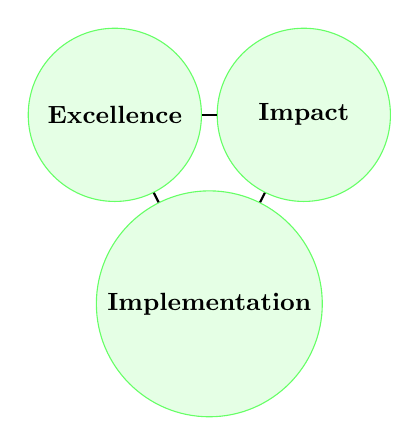
\begin{tikzpicture}[node distance=2.4cm]
			\tikzstyle{crit}=[
			circle, draw=green!60, fill=green!10,
			minimum width=2.2cm, minimum height=2.2cm,
			font=\small\bfseries, align=center
			]
			
			\node[crit] (ex)  {Excellence};
			\node[crit, right of=ex] (im) {Impact};
			\node[crit, below of=ex, xshift=1.2cm] (impl) {Implementation};
			
			\draw[thick] (ex) -- (im);
			\draw[thick] (im) -- (impl);
			\draw[thick] (impl) -- (ex);
		\end{tikzpicture}
		
		\vspace{4pt}
		\small Every proposal is judged on these three \textbf{pillars}.
	\end{frame}
	
	%-------------------------- EXCELLENCE (IDEA) ----------------------------
\begin{frame}{Excellence: The Idea}
	\begin{itemize}
		\item The proposal must start with a \textbf{simple and clear problem}.
		\item It must explain what people \textbf{already know} about this problem.
		\item It must show what is \textbf{missing} or what is not solved yet.
		\item It should have \textbf{clear goals} that the team wants to reach.
		\item The idea should follow a \textbf{logical plan} and make sense.
	\end{itemize}
\end{frame}
	
	%------------------------ EXCELLENCE (METHOD) ----------------------------
\begin{frame}{Excellence: The Method}
	\begin{itemize}
		\item The proposal must show \textbf{how} the team will work.
		\item It should list the \textbf{tools} and \textbf{techniques} they will use.
		\item It must explain \textbf{why} these tools are the right choice.
		\item It should say how they will \textbf{collect} and \textbf{study} data.
		\item It must mention possible \textbf{problems} and how they will solve them.
	\end{itemize}
\end{frame}
	
	%------------------------------- IMPACT ----------------------------------
	\begin{frame}{Impact: The Change}
		\begin{itemize}
			\item Describes what will \textbf{change} if the project is successful.
			\item Links the project to \textbf{EU missions} or strategies.
			\item Explains who will \textbf{benefit} and how.
			\item Gives simple \textbf{numbers} to measure success
			(for example fewer accidents, less energy use).
		\end{itemize}
	\end{frame}
	
	%---------------------------- IMPACT PLANS -------------------------------
	\begin{frame}{Impact Plans: Use and Communication}
		\begin{itemize}
			\item Shows how results will be \textbf{used} after the project
			(for example product, service, policy).
			\item Explains how results will be \textbf{shared}:
			reports, websites, open events, training.
			\item Talks about the \textbf{target groups}:
			cities, companies, citizens, students.
			\item Makes sure the project does not end in a \textbf{drawer}.
		\end{itemize}
	\end{frame}
	
	%---------------------------- IMPLEMENTATION -----------------------------
	\begin{frame}{Implementation: Work Plan}
		\begin{itemize}
			\item Breaks the project into \textbf{work packages}.
			\item Each work package has tasks, a leader and a time period.
			\item Shows a simple \textbf{timeline} (Gantt style).
			\item Explains how partners will \textbf{manage} the project:
			meetings, reports, risk checks.
		\end{itemize}
	\end{frame}
	
	%---------------------------- IMPLEMENTATION 2 ---------------------------
	\begin{frame}{Implementation: The Team}
		\begin{itemize}
			\item A good consortium mixes:
			\begin{itemize}
				\item \textbf{Universities} (knowledge)
				\item \textbf{Companies} (market and products)
				\item \textbf{Cities or users} (real-life testing)
			\end{itemize}
			\item Each partner has a \textbf{clear role}.
			\item The coordinator has experience in \textbf{project management}.
		\end{itemize}
	\end{frame}
	
	%------------------------------- TABLE -----------------------------------
	\begin{frame}{Short Overview of the Three Criteria}
		\centering
		\begin{tabular}{|p{3cm}|p{7cm}|}
			\hline
			\textbf{Excellence} &
			Quality of the idea and method. Clear problem and clear objectives. \\ \hline
			\textbf{Impact} &
			Useful change in society or the market. Strong link to EU goals. \\ \hline
			\textbf{Implementation} &
			Realistic work plan, good team and management. \\ \hline
		\end{tabular}
	\end{frame}
	
	%-------------------------- SMART TRAFFIC IMAGE -------------------------
	\begin{frame}{Example Project: Smart Traffic}
		\begin{columns}
			\begin{column}{0.45\textwidth}
				\includegraphics[width=\textwidth]{images/eu3.jpg}
			\end{column}
			\begin{column}{0.55\textwidth}
				\small
				\begin{itemize}
					\item Goal: make a city \textbf{safer} at busy crossings.
					\item University builds an \textbf{AI model} to predict risky situations.
					\item Company builds \textbf{smart cameras} and software.
					\item City installs the system at real junctions.
				\end{itemize}
			\end{column}
		\end{columns}
	\end{frame}
	
	%-------------------------- SMART TRAFFIC + CRIT ------------------------
	\begin{frame}{Smart Traffic Project and the Criteria}
		\small
		\begin{itemize}
			\item \textbf{Excellence}: clear accident problem, new AI-based solution.
			\item \textbf{Impact}: fewer injuries, supports green and smart city mission.
			\item \textbf{Implementation}: clear work packages,
			3-year plan, partners with real responsibilities.
		\end{itemize}
	\end{frame}
	
	%--------------------------- COMMON MISTAKES -----------------------------
	\begin{frame}{Typical Weak Points in Proposals}
		\begin{itemize}
			\item Problem is \textbf{not clear} or too broad.
			\item Many nice words but \textbf{no concrete impact}.
			\item Work plan looks \textbf{too optimistic} for the time and budget.
			\item Missing important partners (for example no city partner for a city project).
			\item Risks are ignored or only written in one short line.
		\end{itemize}
	\end{frame}
	
	%------------------------- WHAT MAKES IT STRONG --------------------------
	\begin{frame}{What Makes a Proposal Strong}
		\begin{itemize}
			\item Simple and \textbf{clear story} that everyone understands.
			\item Real \textbf{innovation}, but still realistic.
			\item Impact that matches \textbf{EU missions}.
			\item Work plan that looks \textbf{doable}.
			\item Team that has the \textbf{right skills}.
		\end{itemize}
	\end{frame}
	
	%----------------------------- STUDENT IMAGE -----------------------------
	\begin{frame}{Students in EU Projects}
		\begin{columns}
			\begin{column}{0.5\textwidth}
				\includegraphics[width=\textwidth]{images/eu4.jpg}
			\end{column}
			\begin{column}{0.5\textwidth}
				\small
				\begin{itemize}
					\item Students cannot be \textbf{main applicants}.
					\item But they can work inside a \textbf{university team}.
					\item They help with data, coding, tests and reports.
					\item This gives strong \textbf{experience} and a good CV.
				\end{itemize}
			\end{column}
		\end{columns}
	\end{frame}
	
	%--------------------------- STUDENT PATH TIKZ --------------------------
	\begin{frame}{How a Student Can Join a Project}
		\centering
		\begin{tikzpicture}[node distance=1.5cm]
			\tikzstyle{step}=[
			rectangle, draw=purple!70, fill=purple!10,
			rounded corners, minimum width=4cm,
			minimum height=0.9cm, font=\small
			]
			
			\node[step] (interest) {1. Interest in a topic};
			\node[step, below of=interest] (prof) {2. Talk to a professor};
			\node[step, below of=prof] (group) {3. Join a research group};
			\node[step, below of=group] (project) {4. Work on an EU project};
			
			\draw[->, thick] (interest) -- (prof);
			\draw[->, thick] (prof) -- (group);
			\draw[->, thick] (group) -- (project);
		\end{tikzpicture}
	\end{frame}
	
	%----------------------------- STUDENT ROLES -----------------------------
	\begin{frame}{Typical Student Roles}
		\begin{itemize}
			\item \textbf{Data work}: collecting, cleaning and simple analysis.
			\item \textbf{Programming}: small modules, scripts, dashboards.
			\item \textbf{Testing}: trying out prototypes in the lab or in the field.
			\item \textbf{Support}: helping with figures, slides and documentation.
			\item \textbf{Thesis}: writing a project-related bachelor or master thesis.
		\end{itemize}
	\end{frame}
	
	%------------------------------- BENEFITS --------------------------------
	\begin{frame}{Benefits for Students}
		\begin{itemize}
			\item Learn how real \textbf{EU projects} work.
			\item Build an \textbf{international network}.
			\item Gain experience that looks strong on a \textbf{CV}.
			\item Understand how research ideas become \textbf{funded projects}.
		\end{itemize}
	\end{frame}
	
	%------------------------------- SUMMARY ---------------------------------
	\begin{frame}{Summary}
		\begin{itemize}
			\item EU projects are evaluated on \textbf{Excellence}, \textbf{Impact} and
			\textbf{Implementation}.
			\item Only clear, realistic and high-impact proposals are funded.
			\item Students cannot lead these proposals but can \textbf{join} them.
			\item Working in such a project is a strong step for a \textbf{future career}.
		\end{itemize}
	\end{frame}
	
	%--------------------------------- END -----------------------------------
	\begin{frame}
		\centering
		\Large Thank you for listening.\\[8pt]
		\large Questions?
	\end{frame}
	
\end{document}